\labday{Identificação das órbitas periódicas instáveis imersas no atrator apresentado}

\experiment{OPIs identificadas}

Utilizando r1 = 0.3 e r2 = 0.6 foram identificadas as seguintes OPIs.
\\

\begin{center}
$\begin{array}{ccc}
	x(rad)        & y(rad/s)      & n \\  
	4.1 & -0.74 &  1\\ 
	2.1 & -2.04 &  1\\ 
	2.65 & -10.62 &  2\\ 
	6.5 & -6.0 &  2\\ 
	4.17264849349 &  8.0428748441 &  3\\ 
	5.94706541985 & -0.6067772472 &  3\\ 
	2.27480878676 &  2.3392263042 &  3\\ 
	2.45846211242 & -8.0518576316 &  4\\ 
	0.25182552135 &  10.0102125165 &  5\\ 
	5.46130245257 & -13.9295391669&  5\\ 
	0.40502528744 & -14.1037540837&  5\\ 
	0.54618738231 &  -3.09172989752&  5\\ 
	5.58822458831 &  11.3129421811&  5\\ 
	5.54611674952 &  2.71994232771&  6\\ 
	0.94182908055 &  6.91173601164&  6\\ 
	5.28879201165 &  7.61171362826&  6\\ 
	0.67314851499 &  -10.5069349506&  6\\ 
	3.20607450608 &  -2.38651681226&  6\\ 
	4.21389240354 &  1.63170963314&  6\\ 
	5.48445583246 &  -5.08170099625&  6\\ 
	3.16436778537 &  1.90374698997&  6\\ 
	2.20701614324 &  -4.34496029587&  6\\ 
	5.26738222216 &  0.779490648627&  6\\ 
	1.10509496686 &  5.52462297441&  6\\ 
	1.28271281324 &  -14.2296486224&  7\\ 
	5.08748787592 &  12.0889148879& 7
\end{array}$ 
\end{center}

\experiment{Espaços de estado das órbitas identificadas}

Abaixo são apresentados os espaços de estado para cada uma das órbitas identificadas
\\

\textbf{Órbitas de período 1:}

\begin{figure}[!ht]
	\centering
	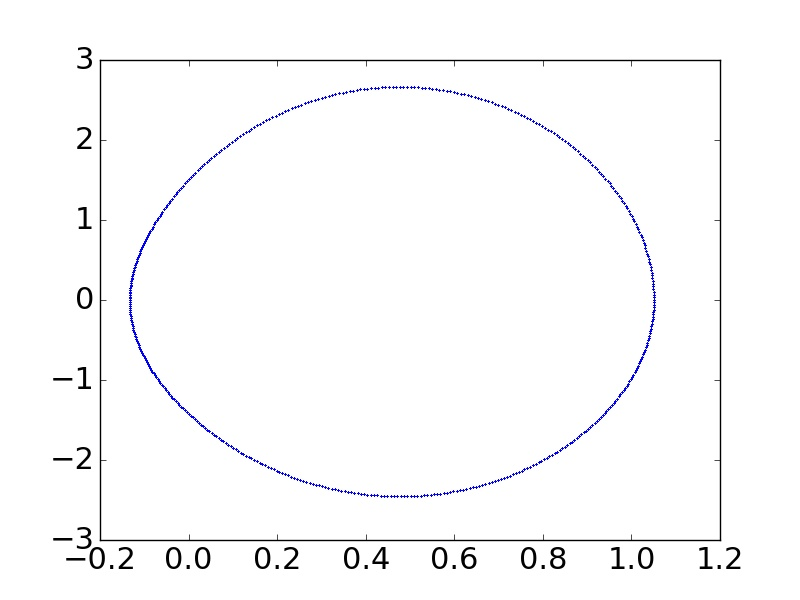
\includegraphics[scale=0.35]{OPI_identification/state_space4,1.jpg}
	\caption{Espaço de estado para um forçamento de 3.41011183943 rad/s}
	\label{state_space_4.1rad/s}
\end{figure}

\begin{figure}[!ht]
	\centering
	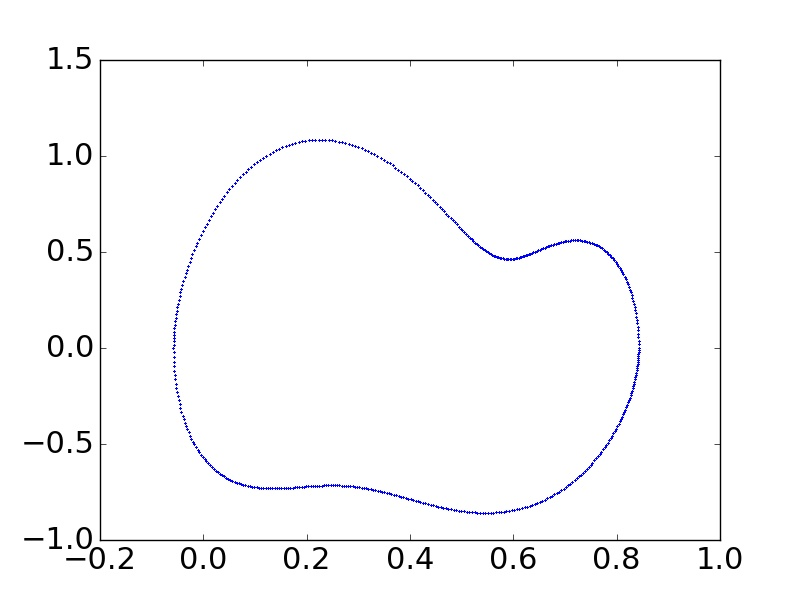
\includegraphics[scale=0.35]{OPI_identification/state_space2,1.jpg}
	\caption{Espaço de estado para um forçamento de 2.1 rad/s}
	\label{state_space_2.1rad/s}
\end{figure}
\hspace{1mm}

\textbf{Órbitas de período 2:}

\begin{figure}[!ht]
	\centering
	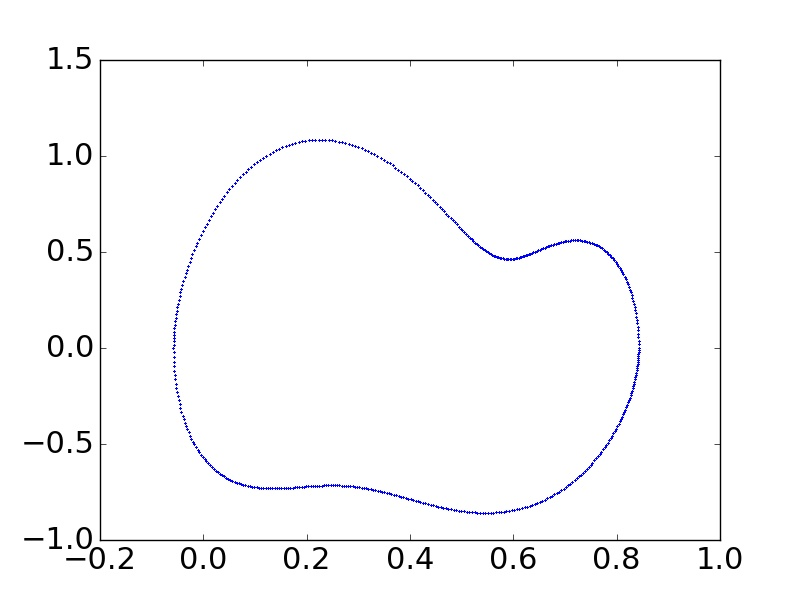
\includegraphics[scale=0.35]{OPI_identification/state_space2,1.jpg}
	\caption{Espaço de estado para um forçamento de 2,65 rad/s}
	\label{state_space_2.65rad/s}
\end{figure}


\begin{figure}[!ht]
	\centering
	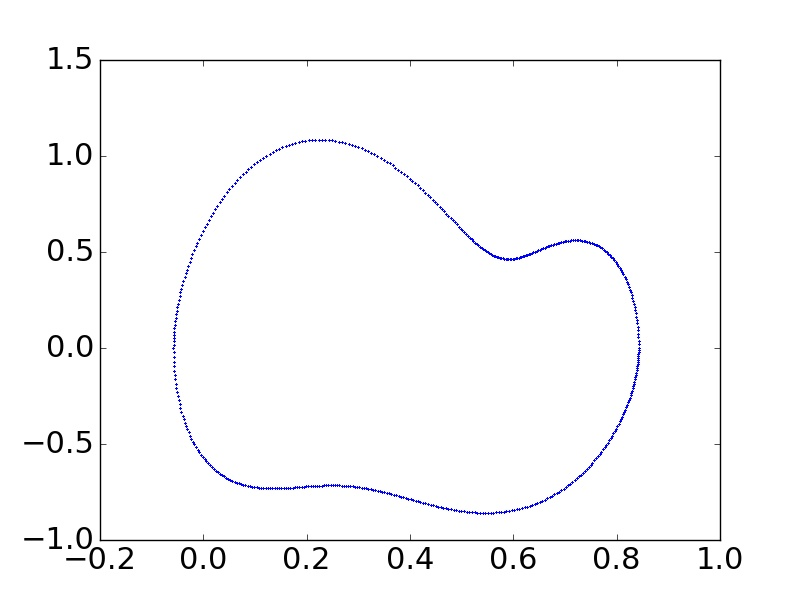
\includegraphics[scale=0.35]{OPI_identification/state_space2,1.jpg}
	\caption{Espaço de estado para um forçamento de 6,5 rad/s}
	\label{state_space_6.5rad/s}
\end{figure}

